Au début de ce stage, le logiciel \textit{symbolist} en est déjà à un état de développement avancé. Cette section détaille l'état de l'application d'un point de fonctionnel, technologique et architectural, tel qu'il se trouvait au début de la période de formation.

\subsection{Interface et fonctionnalités existantes}
\label{subsec:uiAndExistingFeatures}

Au commencement du stage, l'interface graphique de \textit{symbolist} offre déjà les fonctionnalités basiques de dessin sur l'espace de la partition. Les différentes vues composants l'éditeur graphique de \textit{symbolist} sont présentées en figure \ref{fig:symbolistUIBefore}.

\begin{figure}[H]
	\centering
	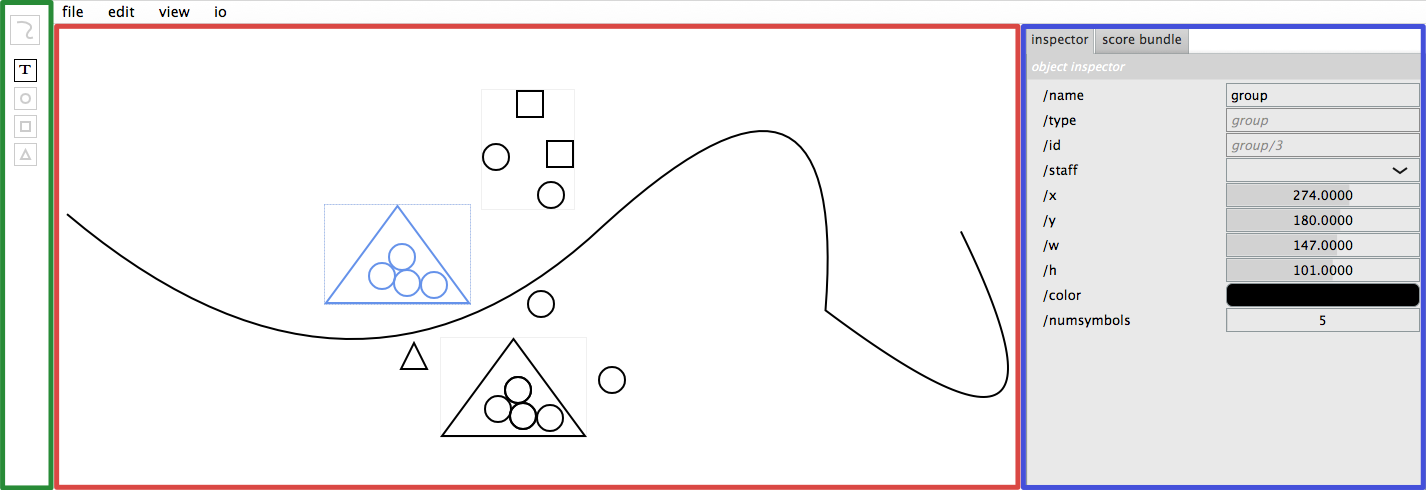
\includegraphics[keepaspectratio=true, width=\textwidth]{PresentationDeSymbolist/i/symbolistUIBefore.png}
	\caption{Éditeur graphique de \textit{symbolist}}
	\label{fig:symbolistUIBefore}
	\small
	\it
	En \textcolor{green}{vert}, la palette des symboles disponibles et dessinables sur la partition. En \textcolor{red}{rouge}, la partition, ou l'espace de composition et d'édition des symboles. En \textcolor{blue}{bleu}, l'inspecteur de symboles, qui présente le bundle OSC associé au symbole graphique couramment sélectionné (symbole surligné en bleu dans la partition).
\end{figure}

L'éditeur graphique de \textit{symbolist} permet à l'utilisateur de dessiner directement sur la partition à l'aide de la souris, dans une modèle d'interaction \textit{wysiwyg} (\textit{what you see is what you get}). Dans \textit{symbolist}, la partition fait référence à l'espace graphique où les symboles sont placés et édités par l'utilisateur. De manière sous-jacente, la partition est stockée comme une liste de symboles. Les symboles de la partition qui sont attachés à un référent temporel, un \textit{staff}, se voient attribuer une valeur temporelle de départ et de fin correspondant à leur point de départ et de fin sur l'axe horizontal. Ces symboles sont ordonnancés temporellement dans la liste reflétant la partition.

De plus, l'éditeur graphique n'est pas le seul moyen d'interagir avec le logiciel \textit{symbolist}. En effet, \textit{symbolist} est également déployer dans une version \textit{objet} pour l'environnement \textit{Max} et l'environnement \textit{OpenMusic}. Dans ces environnements, l'application \textit{symbolist} est représentée comme une boîte, recevant et envoyant des messages à d'autres objets. Les différents messages auxquels répond l'objet \textit{symbolist} dans l'environnement Max sont présentés en figure \ref{fig:symbolistMaxObject}.

\begin{figure}[H]
	\centering
	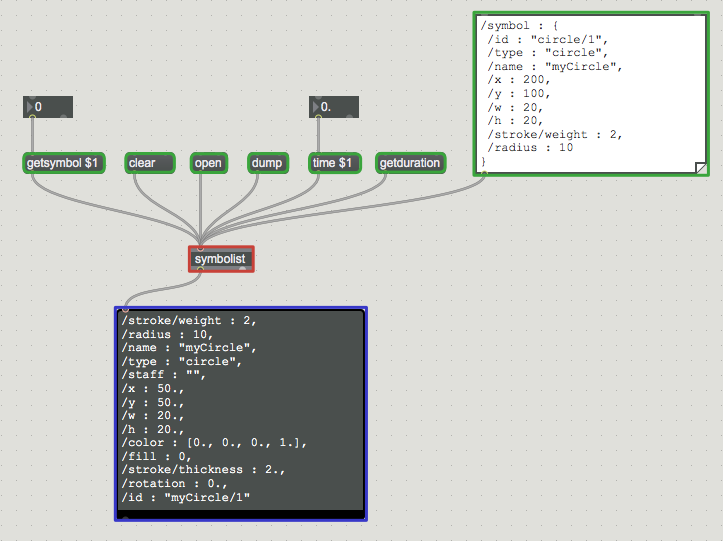
\includegraphics[keepaspectratio=true, width=0.8\textwidth]{PresentationDeSymbolist/i/symbolistMaxObject.png}
	\caption{L'objet \textit{symbolist} dans Max}
	\label{fig:symbolistMaxObject}
	\small
	\it
	En \textcolor{red}{rouge}, l'objet \emph{symbolist} représenté, comme tous les objets \emph{Max}, sous forme de boîte. En \textcolor{green}{vert}, les messages pouvant être envoyés à l'objet \emph{symbolist}.
	En \textcolor{blue}{bleu}, un afficheur de bundle OSC, proposé par une librairie indépendante, témoin des messages de sortie générés par l'objet \emph{symbolist}.  
\end{figure}

Les messages\footnote{Dans Max, un message peut être envoyé à un objet via l'objet \textit{message}, qui n'est autre qu'un bouton cliquable avec un label, à connecter à l'entrée d'un receveur.} compris par l'objet \textit{symbolist} permettent de lire et d'écrire des symboles dans la partition.
Comme exemples de messages de lecture, \lstinline|getsymbol n|, lit le \textit{n-ième} symbole de la partition, \lstinline|time t|, lit le contenu de la partition au temps \textit{t}…
Le résultat de la lecture est envoyé sur la sortie de l'objet \textit{symbolist}.

L'écriture de symboles dans la partition se fait par l'envoi de bundles OSC en entrée de l'objet \textit{symbolist} (voir la figure \ref{fig:symbolistMaxObject}, en haut à droite). 
Enfin, l'éditeur graphique peut être lancé par l'envoi du message \lstinline|open|.

\textit{symbolist} est également déployé dans une version objet \textit{OpenMusic}. La figure \ref{fig:symbolistOMObject} montre un exemple de computation de partition avec l'objet \textit{symbolist} (nommé \textit{sym-score}) dans \textit{OpenMusic}.

\begin{figure}[H]
	\centering
	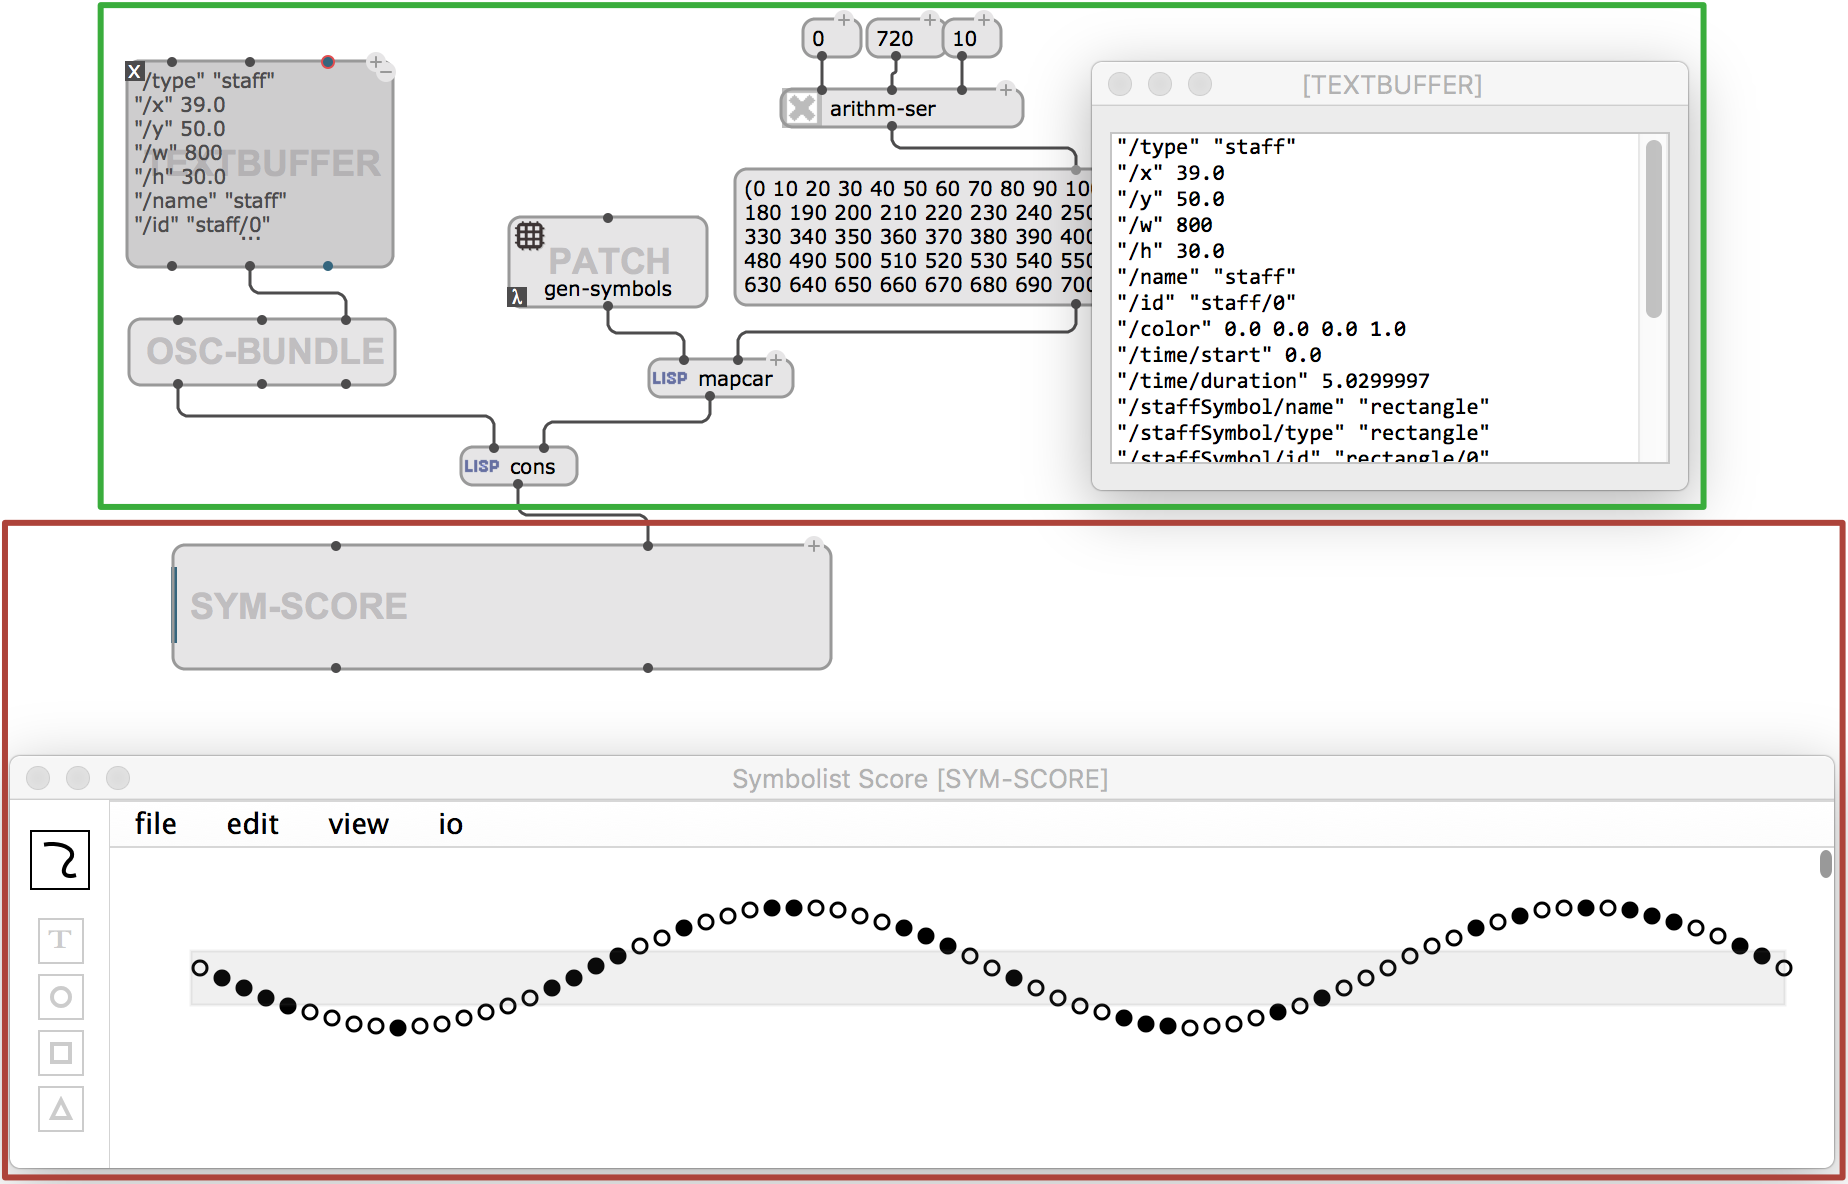
\includegraphics[keepaspectratio=true, width=\textwidth]{PresentationDeSymbolist/i/symbolistOMObject.png}
	\caption{L'objet \textit{symbolist} dans OpenMusic}
	\label{fig:symbolistOMObject}
	\small
	\it
	En \textcolor{red}{rouge}, l'objet \emph{symbolist} \og sym-score \fg et l'éditeur graphique associé.
	En \textcolor{green}{vert}, les objets \emph{OpenMusic} servant à la création de bundles OSC envoyés à l'objet \emph{sym-score}.
\end{figure}

L'objet \textit{symbolist} dans sa version \textit{OpenMusic} reçoit des bundles OSC et crée les symboles correspondant dans la partition. Ensuite, le contenu de la partition peut être envoyé sur la sortie, en utilisant la barre de lecture \textit{OpenMusic} (activée par la touche espace).    

\paragraph{Fonctionnalités existantes} Afin de dresser un bilan des fonctionnalités implantées dans \textit{symbolist}, des \textit{user-stories}\footnote{Une \textit{user-story} est une manière d'exprimer une fonctionnalité logiciel, répandue chez les praticiens de la philosophie Agile. Une \textit{user story} prend la forme: \og En tant que tel type d'utilisateur, j'effectue telle action dans tel but \fg. De cette manière, une fonctionnalité est exprimée du point de vue de l'utilisateur, évitant l'écueil d'une formalisation trop technique. } ont été écrites à partir des possibilités du logiciel.
La liste des \textit{user stories} implantées dans \textit{symbolist} au début du stage est la suivante:
\begin{itemize}[label=--]
	\item En tant que compositeur, je dessine des courbes pour créer de nouveaux symboles.
	\item En tant que compositeur, je dessine des formes géométriques pour créer de nouveaux symboles.
	\item En tant que compositeur, j'écris du texte pour créer de nouveaux symboles ou pour annoter ma partition.
	\item En tant que compositeur, j'édite les propriétés d'un symbole existant pour définir sa forme.
	\item En tant que compositeur, je groupe des symboles entre eux pour créer un nouveau symbole.
	\item En tant que compositeur, je transforme un symbole en \textit{staff}, pour définir une référence temporelle dans la partition.
	\item En tant que compositeur, j'associe un symbole à un \textit{staff} pour lui procurer une valeur temporelle.
	\item En tant que compositeur, je peux ajouter un de mes propres symboles à la palette pour le réutiliser ensuite.
	\item En tant que compositeur, je peux annuler/recommencer les actions effectuées sur la partition pour la maintenir dans une état cohérent.
	\item En tant que compositeur, je peux lire le contenu de ma partition à un temps $t$. 
\end{itemize}

Les \textit{user stories} concernant le dessin sur la partition ont été réparties en catégories. En effet, chaque type de symboles est accompagné de problématiques spécifiques, ce qui fait considérer la création de texte, de courbes ou de formes prédéfinies comme des fonctionnalités à part entière.

\subsection{Framework de développement pour l'application symbolist}
\label{subsec:frameworkAndTechnologies}
\textit{symbolist} est développé avec le framework \textit{C++} \textit{JUCE} \cite{juce2018}. L'environnement \textit{JUCE} est un standard pour le développement d'applications liées à l'audio. Dans le cas de \textit{symbolist}, \textit{JUCE} a été utilisé pour ses capacités de gestion des bundles OSC et création d'interface graphique. La librairie \textit{odot} a ensuite été préférée pour la gestion des bundles OSC dans \textit{symbolist}. En effet, \textit{odot} augmente les capacités du format OSC, en lui adjoignant par exemple un léger langage de programmation. Aujourd'hui \textit{JUCE} n'est donc plus utilisé dans \textit{symbolist} que pour ses composants graphiques. 

En plus de son framework de développement, l'application \textit{symbolist} est également destinée à être déployée dans les deux environnements que sont \textit{Max} et \textit{OpenMusic}. Aussi, la construction de l'application \textit{symbolist} en tant qu'objet \textit{Max} et \textit{OpenMusic} est détaillée ci-après.

\paragraph{Création d'un objet Max} Max propose une API pour la création de nouveaux objets \cite{maxApi2018}. L'API Max est écrite en \textit{C}, ainsi que doivent l'être les objets créés par les utilisateurs pour étendre le système.
Ces objets sont appelés des \textit{externals} dans Max.
Ils doivent posséder une certaine structure pour pouvoir être compilé et utilisé par la suite:
\begin{itemize}[label=--]
	\item Le fichier de définition de l'external doit inclure le header \textit{ext.h} à la première ligne.
	\item Le nouvel objet défini doit être déclaré comme une structure \textit{C} avec un premier champ de type spécial.
	\item Une méthode de création et de libération de l'objet doivent être définies, ainsi qu'une méthode pour chaque message que peut recevoir l'objet.
	\item Ces méthodes sont liées à l'objet au sein de la procédure \lstinline|ext_main| qui fait office de procédure d'initialisation. De fait, \lstinline|ext_main| est appelée lorsque l'objet cible est appelé dans un patch Max, c'est à dire lorsque son nom est tapé dans une boîte.
\end{itemize}

L'application \textit{symbolist} étant implémentée en \textit{C++}, une API équivalente en \textit{C} a été écrite afin de pouvoir communiquer avec \textit{Max} et \textit{OpenMusic}.
Les méthodes fournies par l'API \textit{C} \textit{symbolist} sont présentées en annexe , page .
\todo[inline]{Ajouter l'API C symbolist en annexe}  

\paragraph{Création d'un objet OpenMusic} \textit{OpenMusic} pouvant être vu comme une surcouche graphique du langage \textit{Common Lisp} et de son système objet \textit{CLOS} \cite{bresson2009}, la création de nouveaux objets \textit{OpenMusic} est équivalent à la définition d'une nouvelle classe \textit{Lisp}.
Par exemple, l'objet \textit{symbolist} dans \textit{OpenMusic} est définie comme une classe possédant deux attributs: l'attribut \textit{symbols}, une liste de bundles OSC représentant la partition, et l'attribut \textit{palette-symbols}, une autre liste de bundles OSC représentant la palette des symboles disponibles.  
De fait, la boîte représentant l'objet \textit{symbolist} dans \textit{OpenMusic} possède trois points d'entrée et de sortie. Le premier point d'entrée correspond à la définition par copie d'un objet \textit{symbolist} par un autre objet \textit{symbolist}; le point d'entrée est dénommé \textit{self}. Les deux autres points d'entrées correspondent aux attributs de l'objet \textit{symbolist}, \textit{symbols} et \textit{palette-symbols}.
Les mêmes points se retrouvent symétriquement définis en sortie.

Un objet \textit{OpenMusic} peut également être muni d'un éditeur, c'est à dire une fenêtre graphique apparaissant lors d'un double-clic sur l'objet. L'éditeur associé à un objet \textit{OpenMusic} est défini par une classe \textit{Lisp} étendant la classe \textit{OMEditor}. 
Dans le cas de l'objet \textit{symbolist}, son éditeur fait la liaison avec l'API \textit{C} permettant de contrôler avec l'application \textit{symbolist} et son interface.
 
\subsection{Architecture de l'application symbolist}
\label{subsec:architectureBefore}
Le framework \textit{JUCE}, utilisé pour développer l'application \textit{symbolist}, n'impose pas d'architecture logicielle. Aussi, les applications développées avec ce framework définissent chacune leurs propres structures.
L'architecture logicielle de \textit{symbolist} n'est pas clairement définie au début de ce stage, néanmoins trois parties peuvent être distinguées dans le code source. 

Une première partie est centrée autour de la classe \textit{SymbolistHandler}. Cette classe permet l'accès depuis l'extérieur à l'application \textit{symbolist}. A savoir, l'API \textit{C} permettant à \textit{Max} et \textit{OpenMusic} de communiquer avec \textit{symbolist} appelle les méthodes de la classe \textit{SymbolistHandler} pour pouvoir interagir avec le reste de l'application.

Une deuxième partie correspond aux composants graphiques construisant l'interface de \textit{symbolist}. La fenêtre principale de l'application \textit{symbolist} est représentée par la classe \textit{SymbolistMainComponent}. Cette partie comprend également toute la hiérarchie des composants graphiques représentant les symboles de la partition.

La troisième partie de l'application regroupe les classes du \og cœur métier \fg, représentant la partition et la palette du compositeur. 
S'y trouvent les classes implémentant la structure des bundles OSC, où plus précisément des bundles \textit{odot}, qui définissent le format de données sous-jacent des symboles de la partition.
Pour décrire les symboles de la partition, l'application \textit{symbolist} possède une unique classe \textit{Symbol} (qui hérite de la classe \textit{OdotBundle}). De fait, chaque symbole de la partition, qu'il soit un rond, un carré, une note de musique, ou du texte, est représentée par une instance de la classe \textit{Symbol}. Les spécificités d'un symbole ne sont pas explicitées par sa classe d'appartenance; 
à savoir, le modèle ne prévoit pas de classes \textit{Circle}, \textit{Square} ou \textit{MusicNote}.
En effet, la philosophie de \textit{symbolist} est de conserver l'information des symboles dans les bundles OSC sous-jacents afin de pouvoir distribuer plus facilement les données de la partition.
Les classes du cœur métier incluent également toute la logique d'ordonnancement temporel des symboles associés à un \textit{staff}.
Le diagramme de classes détaillée du cœur métier de l'application \textit{symbolist} est présenté en annexe , page.
\todo[inline]{Ajouter le diagramme de classes du modèle en annexe.}

\paragraph{Problématiques architecturales} Plusieurs aspects posent un problème dans l'architecture de l'application \textit{symbolist} telle qu'elle se trouve au début du stage.

Premièrement, de la description des composantes de l'application \textit{symbolist} se dégage aisément une architecture de type \textit{modèle-vue-contrôleur}. Cependant, les interactions entre composantes et le rôle de chacune d'elles ne sont pas biens définis. Par exemple, la création de symboles dans \textit{symbolist}, de fait l'écriture dans le \textit{modèle}, est trop souvent réalisée par les composants graphiques du système, ce qui est contraire à l'architecture \textit{MVC}. 

Deuxièmement, même si le modèle de l'application \textit{symbolist} place les symboles de la partition à un même niveau dans la hiérarchie des classes (à savoir, il n'existe qu'une seule classe \textit{Symbol}), les composants graphiques sont eux le reflet de la structure de la partition.
C'est à dire, chaque type de composant graphique est représenté par une classe: par exemple, les cercles sont représentés par la classe \textit{CircleComponent}, les rectangles par la classe \textit{RectangleComponent}…
Aussi, comme les symboles de la partition peuvent être groupés afin de créer de nouveaux symboles, le design pattern \textit{Composite} est approprié à la hiérarchie des composants graphiques. 
Or, au début de ce stage, le design pattern \textit{Composite} n'est pas correctement appliqué. 

Troisièmement, la classe \textit{SymbolistHandler}, qui est directement liée à l'API \textit{C} rendant \textit{symbolist} utilisable par d'autres programmes, s'occupe de toutes les interactions avec les vues de l'interface: la palette, la partition, l'inspecteur… Aussi, la classe \textit{SymbolistHandler} est trop encombrée, et les interactions avec des vues spécifiques mériteraient d'être gérées par des contrôleurs spécifiques.   

  